\documentclass[12pt,letterpaper]{article}
\usepackage{pdfpages}
\usepackage{fancyhdr}
\usepackage[colorlinks=true, urlcolor=blue, linkcolor=blue]{hyperref}
\usepackage{graphicx}
\usepackage[top=1.4in, left=0.5in, right=0.5in, bottom=0.8in]{geometry}
\usepackage[T1]{fontenc}
\usepackage{helvet}
\pagestyle{fancy}
\renewcommand{\headrulewidth}{0pt}
\renewcommand{\footrulewidth}{0pt}
\setlength{\parindent}{0em}
\setlength{\parskip}{1em}


\fancyfoot[C]{\setlength{\unitlength}{1in}\begin{picture}(5,0)\put(-1.8,-1){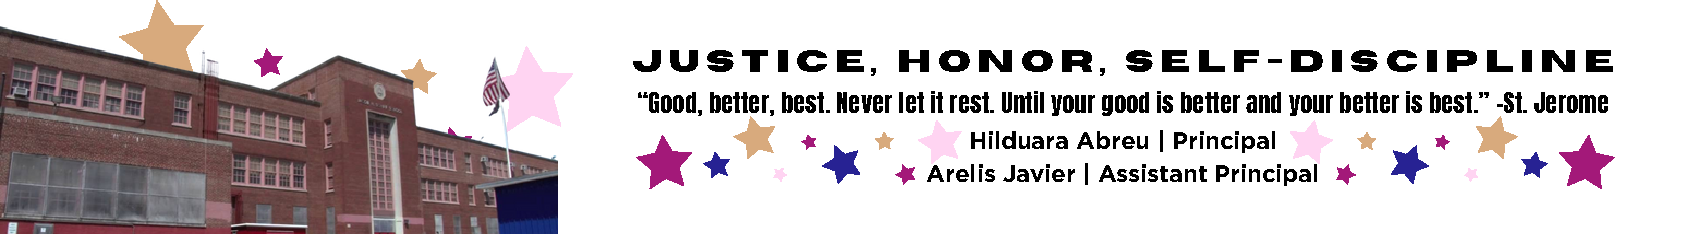
\includegraphics[width=8.8in,height=1.3in]{logo-1}}\end{picture}}
\fancyhead[C]{\setlength{\unitlength}{1in}\begin{picture}(5,0)\put(-1.9,-1){
\includegraphics[width=8.9in,height=1.3in]{logo-2}}\end{picture}}

\pagenumbering{gobble}
\addtolength{\evensidemargin}{-2in}
\addtolength{\topmargin}{-0.5in}
\addtolength{\textwidth}{0in}
%%%%%%%%%%%%%%%%%%%%%%%%%%%%%%%%%%%%%%%%%%%%%%%%%%%%%%%%%%%%%%%%%%

\begin{document}
\vspace*{0.5in}
School Year: \href{https://www.ps192.org}{2024-25} 

\textbf{Subject: School Uniform Policy for P.S. 192}

Dear Parents and Guardians,

We hope this message finds you and your families in good health and high spirits. As we embark on a new
academic year at P.S. 192, we would like to take this opportunity to inform you about our school's uniform policy
and emphasize its importance in fostering a positive and cohesive school community.

At P.S. 192, we believe that a uniform dress code promotes a sense of belonging, equality, and a focused learning
environment. Starting from the academic year 2024-25, the uniform for all students will consist of the following:
\begin{itemize}
	\item Burgundy Shirt: All students are required to wear a burgundy-colored shirt as the upper part of
their uniform.
	\item Navy Pants: Navy blue pants or trousers are to be worn as the lower part of the uniform.
\end{itemize}
The uniform policy will be promoted during school hours and on all school-related events and activities, such as
field trips and special assemblies.

Uniforms serve as a unifying element within our school community and offer several significant advantages:
		\begin{itemize}
		\item Promoting Equality: Uniforms eliminate socioeconomic disparities among students, ensuring that everyone is dressed the same way, regardless of their family's financial circumstances.
		\item Enhancing Focus: Wearing uniforms reduces distractions related to fashion and peer pressure,
allowing students to concentrate on their studies and personal growth.
		\item Fostering School Pride: A uniform instills a sense of pride and belonging among students, helping
them identify with and appreciate their school community.
		\item Improving Safety: Uniforms make it easier to identify intruders in the school premises, enhancing
overall security.
		\item Preparing for Future Success: Encouraging a dress code similar to professional attire helps
prepare students for future careers where a professional appearance is important.
		\end{itemize}
We understand that personal expression is important, and therefore, "Dress Down Days" will be occasionally scheduled throughout the school year, allowing
students to express their individuality through clothing choices.
\pagebreak
\vspace*{1.5cm}
We kindly request your cooperation and support in ensuring that your child
arrives at school dressed in accordance with our uniform policy. We believe that
this will contribute to a more positive and productive learning environment for
all students.

Should you have any questions or concerns regarding the uniform policy, please
feel free to reach out to our Parent Coordinator, Ms Angela Rijo: 
\url{www.ps192.org/angela}, Whatsapp Group, ClassDojo, Phone: (212) 775-9560, or in person during office hours 9:00 AM- 3:00 PM. We are here to assist and support you.

Thank you for your partnership in nurturing a strong and vibrant learning community at P.S. 192. We look forward to a successful and enriching academic year ahead.


In Unity,


\includegraphics[width=0.2\textwidth]{hil_signature}

\textbf{Hilduara Abreu}

\textbf{Principal}

\textit{The School of Joyful Learning!}

\url{www.ps192.org}

\end{document}
